This chapter aims to give an overview of the architecture and structure of the
main components of the project.

\section{Overview}
As previously mentioned, the project is made up of three main parts:
\begin{enumerate}
\item Research Project\\
This project aims to explore the Android Wear APIs and display real world data
obtained from the smartwatch's sensors. Since this project's sole purpose is to
display experimental data, it's user interface is kept minimal and
straight-forward.
\item Wearable Student Application\\
This is the main project of the three and is an application for both
smartwatches and mobile/tablet devices. It's goal is to provide students with
a simple and easy to use app to help them keep track of their lectures and
results whilst also demonstrating some of the newer APIs available in Android
"Lollipop"
\item Calendar Watchface\\
This project provides an example of how to use the new Watchface APIs released
by Google in January 2014. Previously, the APIs were undocumented but a working
prototype was built in the Research Project and was converted to the new
documented APIs in this project.

\end{enumerate}

\section{Application Architecture}
An Android Wear application is bundled with a mobile application. Each
application has it's own \texttt{AndroidManifest.xml} file and
\texttt{res/} directory, but must use the same application id such as
\texttt{com.example.app}. Additionally, the wearable application must declare
the following in it's manifest:
\begin{lstlisting}[language=XML]
<manifest ...>
    ...

    <!-- declare that this is a smartwatch application -->
    <uses-feature
        android:name="android.hardware.type.watch" />

    <application ...>
        ...
    </application>
</manifest>
\end{lstlisting}

The two applications are kept completely separated. As a result, the smartwatch
app does not have access to resources or code of the mobile application and
vise-versa. This can however be achieved using the Gradle build system and
compiling one project as a module of the other project's \texttt{build.gradle}
file. This can be especially useful when serializing objects and sending them
from one application to the other at runtime and not having to duplicate the
code.

\begin{figure}
    \centering
    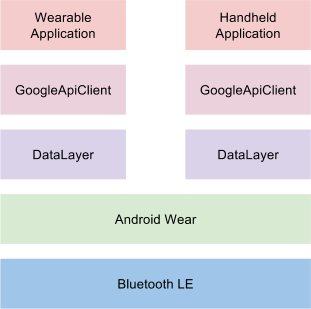
\includegraphics[width=0.7\textwidth]{wear-architecture.png}
    \caption{Application Architecture}
    \label{fig:app_structure}
\end{figure}

When publishing the applications to the Google Play Store, a single APK is
permitted. The Gradle build system will generate a single APK for the handheld
application with the wearable application embedded inside the \texttt{raw}
directory. When installing this APK onto a device, it should automatically
transfer and install the wearable APK on the wearable device.

In order for the two applications to communicate, they use the DataLayer
provided by Android Wear. The DataLayer is accessed via a
\texttt{GoogleApiClient} which can be used to connect Google various APIs,
wearable being one of them. The structure of the application is shown in Figure
\ref{fig:app_structure}

\subsection{Module Structure}

An Android application is comprised of multiple modules. Most mobile
applications wwould only contain a mobile module, but with the introduction of
Android TV, Auto and Wear, modules may be added to support each type of device.
This project only caters for mobile and Android Wear and so consists of two
main modules: one for the mobile application and one for the wearable
application. Modules can also be added to share code between the other modules.
In the case of this project a "common" module was created and added as a
dependancy of the "mobile" and "wear" modules. This allows code as well as
resources such as images and layouts to be shared between the two modules.

\begin{figure}
    \centering
    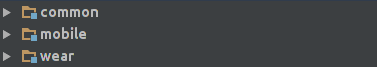
\includegraphics[width=1\textwidth]{module-structure.png}
    \caption{Modules as shown in Android Studio}
    \label{fig:desktop_module_structure}
\end{figure}

The resulting structure is illustrated by Figure
\ref{fig:desktop_module_structure}. Other libraries could also be included here
as modules in Android Studio and get compiled and linked as part of the build
process using Gradle.

Each module is an Android library project. This means that they each follow the
Android project architecture shown in figure \ref{fig:android_project}.

\begin{figure}
    \centering
    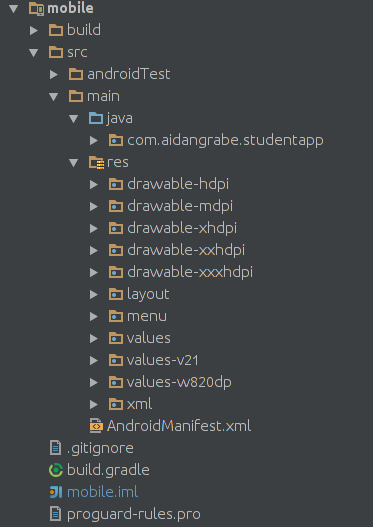
\includegraphics[width=0.6\textwidth]{android-project.png}
    \caption{Android project structure}
    \label{fig:android_project}
\end{figure}

\subsection{Package Overview}

The package structure of the Student Application is quite straight-forward. Each
module follows the basic package structure as shown below:

\begin{description}
\item[adapters] - Contains \texttt{Adapter} classes for dealing with the data
    used by \texttt{ListView}s and \texttt{RecyclerView}s.
\item[activities] - Contains the applications Activity classes.
\item[fragments] - Contains the applications Fragments which are used by the
    Activities.
\item[models] - Contains simple classes that contain mostly attributes eg.
    Module, ToDoItem etc.
\item[tasks] - Contains \texttt{AsyncTask}s that run tasks in the background.
\item[util] - Contains classes that provide utility methods such as
    \texttt{ArrayUtil} ot \texttt{ColorUtil}.
\item[views] - Contains any custom view classes.
\end{description}

If a class is only ever used in a single module, it resides in that module. If
a class needs to be used in both modules, it resides in the common module. This
allows objects to be serialized across the connection and deserialized on the
other side.

\section{Problem Analysis}

This section analyzes the problems faced by building an application for a
handheld device and a wearable, along with the proposed solutions.

\subsection{Communication}

A fundamental part of the application is to communicate from the handheld
application to the wearable application and vice-versa. Reliability, integrity
and confidentiality are all key factors when discussing communication. Bluetooth
is used as the communication layer for Android Wear and by default is not
reliable or secure. Thankfully the Android Wear APIs build these features on top
of the standard Bluetooth protocol. All communications over Bluetooth using the
Android Wear APIs for communication are secured. At the time of writing the
documentation is not clear on how it is secured.

In order to keep communications reliable, we have two options. Use Android
Wear's DataApi or to use the MessageApi. The DataApi is slightly less efficient
as it has more overheads for syncing the data and making sure only objects that
need to be sent are transferred via Bluetooth, but it comes with reliability
built-in. If the wearable is not in range when the handheld application stores
objects using the DataApi, the system buffers the messages until it can reliably
transfer the objects to the wearable when it comes back in range.

The MessageApi does not guarantee reliability. In this case it is up to the
programmer to handle the cases where messages are not delivered and resend them
if neccessary. As a result, if a message needs to be sent reliably in this
project, it is sent using the DataApi. The MessageApi is kept for messages where
reliability is not critical.

\subsection{Synchronizing Data}

Another problem that arises when two applications need to display the same data
set is keeping the data sets on either side in sync. Luckily, the Android Wear
developers have built this straight into the APIs with the DataApi. The DataApi
will automatically replicate changes to a data set on both sides of the
connection. It is up to the programmer to then handle the changes and store
them somewhere on the device.

In this project, the handheld device will act as a server and the wearable as a
client. The wearable will request resources using the MessageApi whenever it
needs them. This prevents the wearable from having to keep the data in sync with
the handheld everytime a change is made to the data set. This also means the
wearable does not have to store any information on the device itself. Since the
wearable has less memory and slower disk access times, it makes sense to leave
the storage to the handheld device.

\subsection{Availability}

With this server-client architecture, the wearable will not be able to display
much information to the user without being connected to the handheld. This is
a problem faced by all client-server models. There is no solution to this
problem, but measures can be taken to lessen it's impact such as caching
information to display when there is no connection. However, this raises further
problems of how and when to refresh this cached data. Cached data might also
give the user a false impression that a connection is available, and frustrate
them by not displaying the latest information.

Alternatively, simply showing a message to the user that a connection is not
available or that the handheld is not in range might be the cleanest solution.
Many features of the wearable are only available when in range of the handheld,
so this project's application would be no different. It also might prompt the
user to rectify the problem, if they can just go pick up their handheld, not
having realized it was too far away to communicate with, it would solve the
problem entirely.

\section{User Interface}

The user interface for this application uses the standard Android SDK, along
with some custom views implemented by drawing on a \texttt{Canvas} object.
The main menu for the handheld is a \texttt{ListView} with custom layouts
for each of the items.

The User Interface for the wearable application uses a \texttt{WearableListView}
which is very similar to a regular \texttt{ListView} but also ensures that the
list's items are not truncated when displayed on a circular screen. The input
is also slightly different in that one item always snaps to the center of the
screen making it easier to select on a small screen.

The watch face application displays an analog clock using the Canvas, but cannot
take input as it is the watch's homescreen and so input is handled by the system
for launching apps and starting voice commands etc.

Due to the amount of screens and different user interfaces throughout the
applications, they will not all be discussed. Most of the handheld UIs are based
on the \texttt{ListView} however, and the wearable's screens are mostly based
on the \texttt{WearableListView} or just the regular \texttt{ListView} in some
places. These screens are also discussed in more detail in next section.

\subsection{Compatibility}
Since Android Wear uses the same base version of Android as phones and tablets,
applications are written in Java and configured using XML just like on mobile.
Most layouts and views work without any changes, however some input fields such
as \texttt{EditText}s are useless since the screen is too small to comfortably
fit a keyboard.\\
Instead of requesting input from a user in the form of text fields, it is
favourable to use speech recognition to allow the user to input textual data.
Some layouts and views are specific to Android Wear such as
\texttt{WatchViewStub}, which allows the developer to select different layouts
for square and circular screens.

At the time of writing there are multiple circular screen devices on the market
such as the first circular smartwatch, the "Moto 360" from Motorola and the "G
Watch R" from LG. By default, layouts will work on both rectangular and
circular screens, but text/parts of the User Interface (UI) may be clipped
depending on radius of the screen and the pixel density.

When creating layouts and user interfaces for a wearable, special care must be
taken to ensure buttons/targets are large enough to be easy to use without
accidentally touching the wrong place, but also to ensure that all elements fit
on the screen for both rectangular and circular screens. Oftern times this means
using a different layout for rectangular screens and circular ones.
